\documentclass[10pt,a4paper]{article}
\usepackage[utf8]{inputenc}
\usepackage[T1]{fontenc}
\usepackage[italian]{babel}
\usepackage{lmodern}
\usepackage[margin=2.2cm]{geometry}
\usepackage{amsmath,amssymb}
\usepackage{graphicx}
\usepackage{booktabs}
\usepackage{tabularx}
\usepackage{xcolor}
\usepackage{tikz}
\usetikzlibrary{arrows.meta,positioning,fit,backgrounds}
\usepackage[hidelinks]{hyperref}
\usepackage{caption}
\captionsetup{font=small,labelfont=bf}
\graphicspath{{figs/}}

\newcommand{\WER}{\mathrm{WER}}
\definecolor{bl}{HTML}{2a6f97}
\definecolor{or}{HTML}{e07a5f}
\definecolor{gr}{HTML}{3d9970}
\definecolor{vi}{HTML}{8e6c8a}

\title{Decodificare il linguaggio dall'attività corticale:\\
una pipeline di machine learning per il Brain-to-Text Benchmark~'24}
\author{Alessandro Saccoia\\\small Università degli Studi di Milano\\\small\textit{Bozza di lavoro, \today}}
\date{}

\begin{document}
\maketitle

\begin{abstract}
Una persona con SLA non riesce più a parlare in modo comprensibile, ma la sua corteccia motoria continua a mandare i comandi per muovere bocca e lingua. Quattro piccoli sensori impiantati registrano quei comandi mentre lei prova a dire frasi mostrate su uno schermo. Il \emph{Brain-to-Text Benchmark '24} (EvalAI, sfida 2099) chiede di ricostruire il testo dalle sole registrazioni, su 1200 frasi di cui non si conosce la trascrizione. Questo documento spiega in modo semplice come è fatto l'esperimento, che cosa impara il modello e come lavora la pipeline che stiamo costruendo: una rete neurale ricorrente (o un Transformer) addestrata con la loss CTC riconosce i fonemi, un modello linguistico 5-gram li trasforma in frasi candidate e un modello linguistico di grandi dimensioni (LLM) sceglie la più sensata. Riportiamo i primi risultati e il piano per avvicinarci al primo classificato (2{,}99\% di parole sbagliate).
\end{abstract}

\section{L'esperimento}

La partecipante T12 fa parte del trial clinico BrainGate2. Ha la sclerosi laterale amiotrofica (SLA): capisce, pensa e legge normalmente, ma i muscoli della parola sono quasi paralizzati. Willett et al.\ (\emph{Nature}, 2023) le hanno impiantato quattro \emph{array Utah}, piastrine di 3\,mm di lato con 64 aghi-elettrodo ciascuna (Fig.~\ref{fig:esperimento}, \textbf{30}):
\begin{itemize}\setlength\itemsep{0pt}
\item due nell'\textbf{area 6v} (\textbf{16}), la zona della corteccia premotoria che comanda i movimenti di labbra, lingua e laringe;
\item due nell'\textbf{area 44} (\textbf{18}), parte dell'area di Broca. In pratica da qui arriva poca informazione utile.
\end{itemize}

\paragraph{Una prova.} Sullo schermo compare una frase (\textbf{10}), per esempio \emph{``i'm sure there are some''}. Dopo una breve attesa arriva il segnale di via e T12 prova a pronunciarla, ad alta voce come riesce oppure muovendo solo le labbra (\textbf{14}). La prova finisce quando lei segnala di aver concluso (\textbf{12}).

\paragraph{Che cosa si registra.} Un connettore sul cranio (\textbf{20}) porta i segnali a un amplificatore che li campiona a 30\,kHz (\textbf{22}). Ogni elettrodo capta l'attività elettrica di pochi neuroni vicini. Quando un neurone ``spara'', la tensione ha un picco rapido verso il basso (\textbf{24}). Per ogni elettrodo e ogni intervallo di 20\,ms si calcolano due numeri (\textbf{26}):
\begin{itemize}\setlength\itemsep{0pt}
\item i \textbf{threshold crossings}: quante volte la tensione è scesa sotto una soglia, cioè circa quanti spari ci sono stati;
\item la \textbf{spike-band power}: quanta energia c'è nelle alte frequenze, una misura più continua della stessa attività.
\end{itemize}
Ogni frase diventa così una tabella di numeri $X$ (\textbf{28}): una riga ogni 20\,ms, una colonna per ogni elettrodo e tipo di misura. Una frase dura da 2 a 20 secondi, cioè da 100 a 1000 righe. Come la baseline, usiamo 256 colonne: le due misure sui 128 elettrodi dell'area 6v. La Fig.~\ref{fig:neural} mostra una di queste tabelle: a occhio non si riconosce nessun fonema.

\begin{figure}[t]
\centering
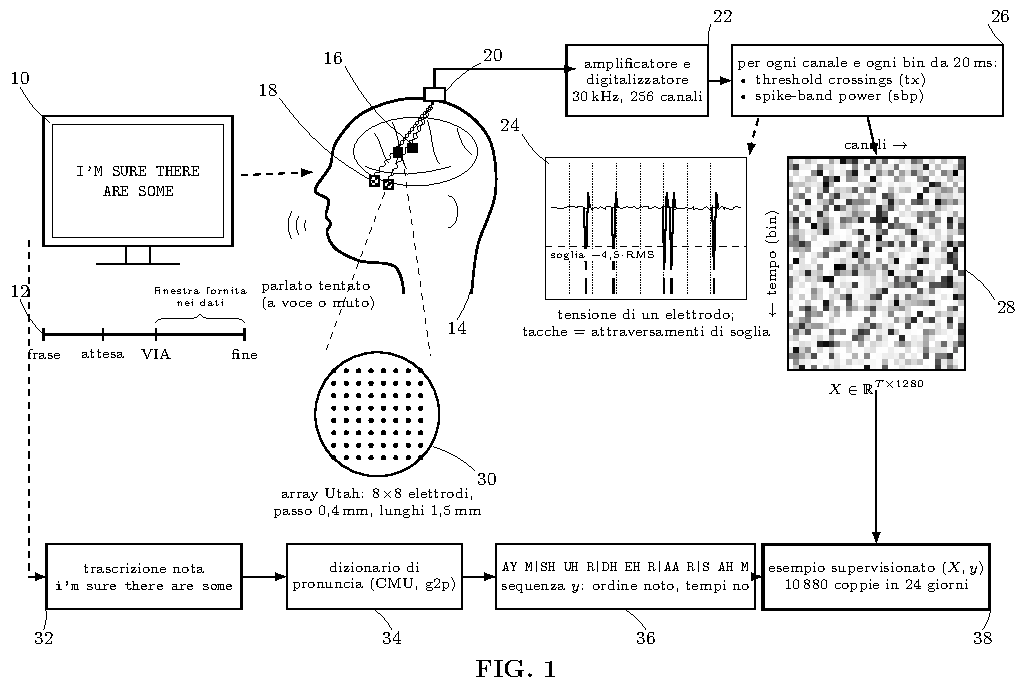
\includegraphics[width=\linewidth]{fig_esperimento.pdf}
\caption{L'esperimento. \textbf{10}~frase mostrata sullo schermo; \textbf{12}~tempi di una prova: nei dati c'è solo la finestra dal via alla fine; \textbf{14}~la partecipante prova a parlare; \textbf{16}, \textbf{18}~array nelle aree 6v e 44; \textbf{20}~connettore; \textbf{22}~amplificatore; \textbf{24}~segnale di un elettrodo, con gli attraversamenti di soglia; \textbf{26}~estrazione delle misure ogni 20\,ms; \textbf{28}~matrice $X$ della frase; \textbf{30}~ingrandimento di un array; \textbf{32}--\textbf{36}~la frase viene trasformata in fonemi con un dizionario di pronuncia; \textbf{38}~ogni prova dà un esempio di addestramento $(X,y)$.}
\label{fig:esperimento}
\end{figure}

\begin{figure}[t]
\centering
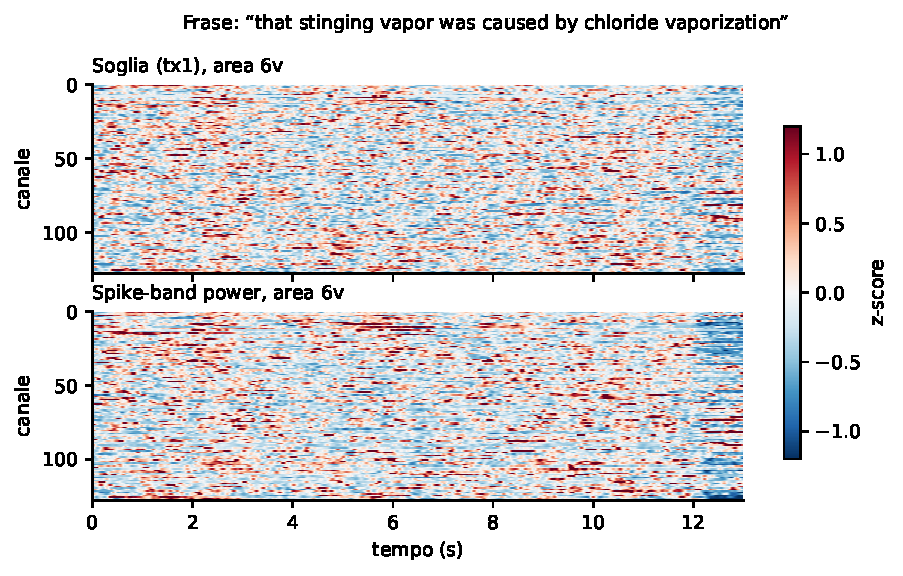
\includegraphics[width=0.92\linewidth]{neural_example.pdf}
\caption{La matrice $X$ di una frase del test (128 dei 256 canali usati per ciascuna misura), normalizzata e smussata. Il segnale è molto rumoroso e la struttura legata ai fonemi non si vede a occhio: per questo servono modelli addestrati su migliaia di frasi.}
\label{fig:neural}
\end{figure}

\paragraph{Quanti dati.} Le 12\,100 frasi sono state registrate in 24 giorni nell'arco di circa quattro mesi (Fig.~\ref{fig:dataset}). Vengono da conversazioni telefoniche (corpus Switchboard) e da testo web, con un vocabolario molto ampio. Gli organizzatori le hanno divise così: 8800 per l'addestramento (\emph{train}), 880 per la verifica (\emph{test}), entrambe con il testo, e 1200 per la gara, senza testo. La gara valuta il \emph{word error rate}, cioè la percentuale di parole sbagliate, aggiunte o mancanti:
\begin{equation}
\WER = \frac{\text{sostituzioni} + \text{inserzioni} + \text{cancellazioni}}{\text{parole della frase vera}}.
\end{equation}
Al 22 novembre 2026 il primo classificato ha il 2{,}99\% e la baseline ufficiale il 9{,}76\%. La gara chiude il 13 gennaio 2027 e accetta al massimo cinque invii al giorno.

\begin{figure}[t]
\centering
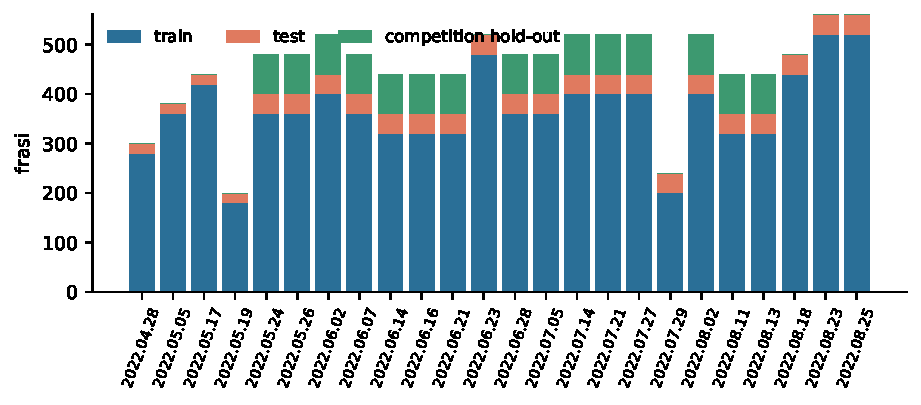
\includegraphics[width=0.92\linewidth]{dataset_days.pdf}\\[2pt]
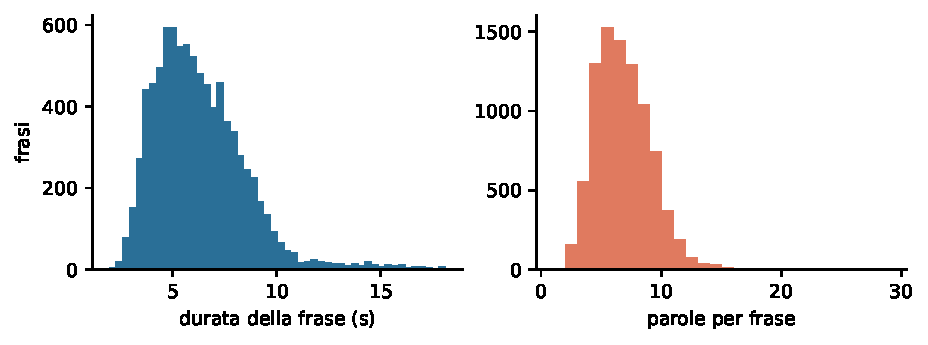
\includegraphics[width=0.92\linewidth]{dataset_hist.pdf}
\caption{In alto: frasi per giorno di registrazione e per partizione. In basso: durata delle frasi del train e numero di parole per frase.}
\label{fig:dataset}
\end{figure}

\section{Che cosa impara il modello}

\paragraph{Apprendimento supervisionato.} Per ogni prova del train sappiamo quale frase T12 doveva dire, perché era sullo schermo. Gli esempi sono quindi coppie (attività neurale $X$, frase), e il modello impara a passare dalla prima alla seconda.

\paragraph{Perché i fonemi.} Il modello non produce direttamente parole ma \textbf{fonemi}, i suoni elementari della lingua: 39 per l'inglese, più un simbolo \texttt{SIL} per la pausa fra parole. La frase viene convertita con un dizionario di pronuncia (Fig.~\ref{fig:esperimento}, \textbf{34}): \emph{``i'm sure''} diventa \texttt{AY M | SH UH R}. Le parole sono decine di migliaia e molte compaiono una sola volta nel train. I fonemi invece sono pochi, compaiono di continuo e corrispondono a movimenti della bocca, cioè proprio a ciò che l'area 6v comanda.

\paragraph{Il problema dei tempi.} L'etichetta dice \emph{quali} fonemi ci sono e in che ordine, ma non \emph{quando} vengono pronunciati (\textbf{36}). Nessuno ha segnato l'istante di ogni fonema, ed è impossibile farlo: dalla bocca di T12 non esce un parlato chiaro da allineare. Non c'è nemmeno un rilevatore di inizio parola (\emph{onset detection}): l'inizio e la fine della frase sono dati dal segnale di via e dalla fine della prova (\textbf{12}), e dentro quella finestra il modello deve capire da solo dove cadono i fonemi. È esattamente il problema che risolve la CTC (Sez.~\ref{sec:ctc}).

\paragraph{Deriva fra giorni.} Da un giorno all'altro gli elettrodi si spostano di qualche micron, alcuni neuroni smettono di essere registrati e altri compaiono. Lo stesso fonema produce quindi tabelle un po' diverse in giorni diversi, e il modello deve tenerne conto.

\section{Il modello}
\label{sec:model}

La Fig.~\ref{fig:modello} mostra tutta la catena. Nelle BCI si chiama \emph{decoder} il sistema che traduce l'attività neurale in testo. Non va confuso con la parte ``decoder'' dei modelli encoder--decoder.

\begin{figure*}[t]
\centering
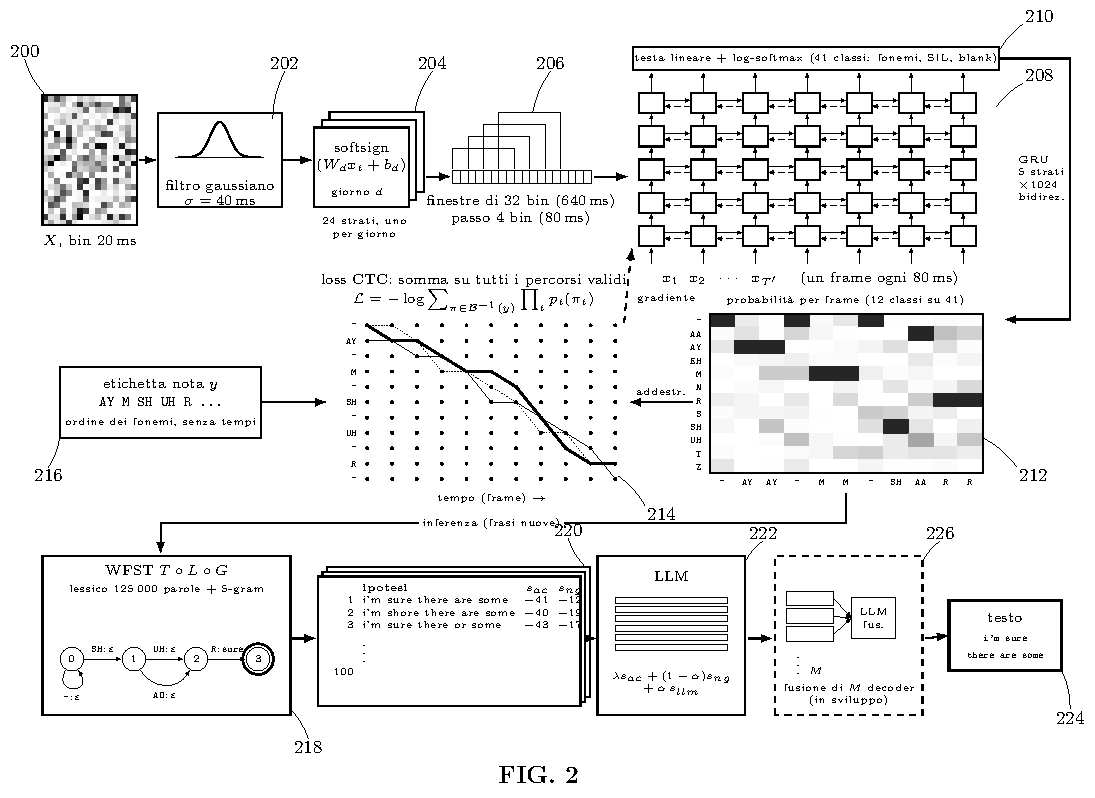
\includegraphics[width=\linewidth]{fig_modello.pdf}
\caption{Il modello. \textbf{200}~matrice $X$; \textbf{202}~smussamento nel tempo; \textbf{204}~strato di correzione specifico per ciascun giorno; \textbf{206}~finestre di 640\,ms ogni 80\,ms; \textbf{208}~rete ricorrente bidirezionale srotolata nel tempo (frecce continue: memoria in avanti; tratteggiate: all'indietro); \textbf{210}~classificatore che a ogni frame dà le probabilità di 41 simboli; \textbf{212}~probabilità per frame (in nero il simbolo più probabile); \textbf{214}~in addestramento la loss CTC confronta queste probabilità con l'etichetta \textbf{216} sommando su tutti gli allineamenti possibili (tre mostrati); \textbf{218}--\textbf{222}~in inferenza un trasduttore con dizionario e modello 5-gram propone 100 frasi, che un LLM riordina; \textbf{226}~fusione di più decoder, in sviluppo; \textbf{224}~testo finale.}
\label{fig:modello}
\end{figure*}

\paragraph{1. Preparazione del segnale (200--206).} Ogni colonna di $X$ viene normalizzata e smussata nel tempo con un filtro gaussiano di 40\,ms, che riduce il rumore dei conteggi (\textbf{202}). Poi passa per uno strato lineare diverso per ciascuno dei 24 giorni, $\tilde x_t=\mathrm{softsign}(W_d x_t+b_d)$ (\textbf{204}). Questo strato impara a correggere la deriva di quel giorno, mentre il resto della rete è uguale per tutti. Infine si raggruppano 32 righe consecutive (640\,ms) ogni 4 righe (\textbf{206}): la rete riceve un ``frame'' ogni 80\,ms, ciascuno con un po' di contesto.

\paragraph{2. La rete ricorrente (208).} Una \textbf{RNN} legge i frame uno dopo l'altro e tiene una memoria interna che si aggiorna a ogni passo. Il suono di un fonema dipende da quelli vicini, quindi questa memoria è essenziale. La baseline usa una \textbf{GRU}, una RNN con ``porte'' che decidono che cosa ricordare e che cosa dimenticare: 5 strati da 1024 unità, letti in tutte e due le direzioni del tempo (bidirezionale), per circa 134 milioni di parametri. Addestriamo anche dei \textbf{Transformer}, che al posto della memoria usano l'\emph{attention}: ogni frame guarda direttamente tutti gli altri e decide quali contano. Sono più piccoli (13--25 milioni di parametri) e nei nostri test imparano più in fretta.

\paragraph{3. Il classificatore (210--212).} A ogni frame uno strato lineare con softmax trasforma l'uscita della rete in 41 probabilità: 39 fonemi, \texttt{SIL} e un simbolo speciale, il \emph{blank} ``--'', che vuol dire ``qui non comincia niente di nuovo''. La Fig.~\ref{fig:ctc} mostra queste probabilità su una frase vera.

\paragraph{Contro il sovradattamento.} Con 8800 frasi la rete rischia di imparare a memoria il train. La rendiamo robusta disturbando gli esempi durante l'addestramento:
\begin{itemize}\setlength\itemsep{0pt}
\item \textbf{rumore}: casuale su ogni valore, e uno spostamento costante per frase e canale, che simula la deriva fra giorni;
\item \textbf{mascheramento nel tempo}: si cancellano tratti casuali fino a metà della frase, e la rete impara a usare il contesto. Con questa tecnica Feghhi et al.\ (2025) hanno portato un Transformer da 11{,}1\% a 8{,}2\% di WER;
\item \textbf{speckle}: si azzerano valori singoli a caso, così la rete non dipende da un solo elettrodo;
\item \textbf{dropout}: si spengono neuroni artificiali a caso dentro la rete.
\end{itemize}

\section{La CTC: imparare senza sapere i tempi}
\label{sec:ctc}

La rete produce un simbolo per frame, quindi una sequenza molto più lunga della frase, per esempio
\begin{center}\small\texttt{-- AY AY -- M M -- SH UH R R}\end{center}
La regola per leggerla è semplice: si uniscono le ripetizioni e si tolgono i blank, e resta \texttt{AY M SH UH R}. Il blank serve anche a separare due fonemi uguali consecutivi.

In addestramento sappiamo che la risposta giusta è \texttt{AY M SH UH R}, ma non quale sequenza lunga la produce: \texttt{AY AY -- M ...}, \texttt{-- AY M M ...} e moltissime altre vanno tutte bene. La \emph{Connectionist Temporal Classification} (Graves et al., 2006) non sceglie: somma la probabilità di \emph{tutti} gli allineamenti validi e chiede alla rete di rendere grande quella somma. Nella Fig.~\ref{fig:modello} (\textbf{214}) ogni percorso dall'alto a sinistra al basso a destra del traliccio è un allineamento. Formalmente, se $\mathcal{B}$ è la regola di lettura,
\begin{equation}
\mathcal{L}_{\text{CTC}} = -\log \sum_{\pi:\ \mathcal{B}(\pi)=y}\ \prod_{t} p_t(\pi_t),
\end{equation}
e la somma si calcola in modo efficiente con la programmazione dinamica. Durante l'addestramento la rete scopre da sola dove cadono i fonemi: la Fig.~\ref{fig:ctc} mostra picchi stretti sui fonemi separati da lunghi tratti di blank. È la stessa tecnica dei riconoscitori vocali di qualche anno fa.

\begin{figure}[t]
\centering
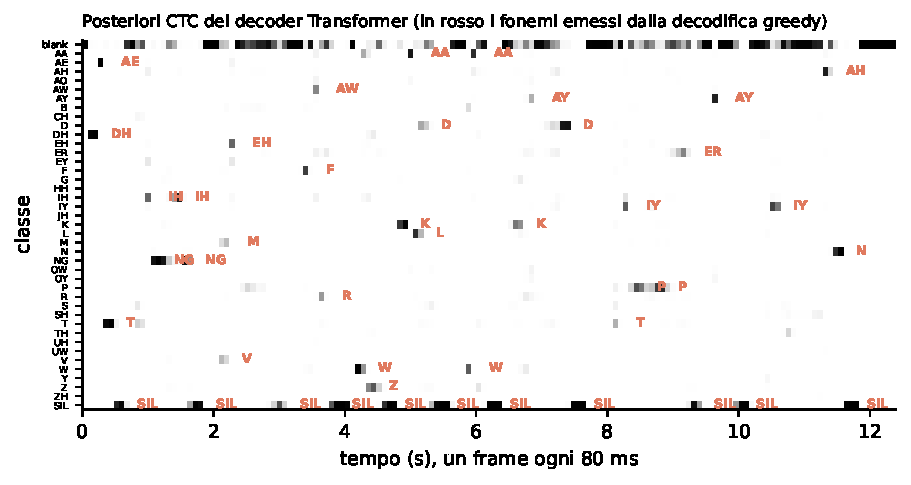
\includegraphics[width=0.95\linewidth]{ctc_posteriors.pdf}
\caption{Probabilità delle 41 classi nel tempo per la frase della Fig.~\ref{fig:neural} (\emph{``that stinging vapor was caused by chloride vaporization''}), da un modello Transformer ancora in addestramento (passo 2500 di 20\,000). Più scuro vuol dire più probabile. In rosso il simbolo scelto in ogni frame, tolti blank e ripetizioni.}
\label{fig:ctc}
\end{figure}

\section{Dai fonemi alle parole}

I fonemi riconosciuti contengono errori. Un modello del linguaggio sa quali frasi inglesi sono probabili e può correggerli. È lo stesso principio del riconoscimento vocale:
\begin{equation}
\text{frase migliore} = \arg\max_W \big[\lambda\cdot\text{(quanto i fonemi spiegano $W$)} + \text{(quanto $W$ è probabile in inglese)}\big].
\label{eq:bayes}
\end{equation}

\paragraph{5-gram (218, 220).} Gli organizzatori forniscono un grafo pesato (WFST) che unisce tre elementi: la regola di lettura della CTC, un dizionario di 125\,000 parole con la loro pronuncia e un modello \textbf{5-gram}, cioè le statistiche su quali parole seguono le quattro precedenti. Una ricerca su questo grafo (44\,GB su disco, circa 94\,GB in memoria) trova le 100 frasi che massimizzano l'Eq.~\eqref{eq:bayes}. Ognuna ha un punteggio neurale $s_{ac}$ e uno linguistico $s_{ng}$. Ci vogliono circa 0{,}3\,s per frase.

\paragraph{LLM (222).} Il 5-gram vede solo quattro parole indietro. Un LLM legge invece la frase intera e ne valuta senso e grammatica. Per ognuna delle 100 frasi calcoliamo la probabilità $s_{llm}$ secondo OPT-6.7B (compresso a 8 bit per entrare in una GPU T4) e scegliamo
\begin{equation}
\hat h = \arg\max_h \big[\lambda\, s_{ac}(h) + (1-\alpha)\, s_{ng}(h) + \alpha\, s_{llm}(h)\big],
\end{equation}
con $\lambda$ e $\alpha$ tarati sul test.

\section{Ensemble e fusione con LLM}

Secondo il report degli organizzatori sulla gara 2024, il miglioramento più grande è venuto dal combinare molti decoder. Il vincitore (DCoND-LIFT) è passato da 8{,}1\% a 5{,}8\% di WER dando a un LLM addestrato le dieci frasi candidate di dieci modelli diversi, insieme alle relative sequenze di fonemi, e chiedendogli di scrivere la frase corretta. Il sistema impara così che tipo di errori fanno i decoder neurali: fonemi simili scambiati, parole spezzate, omofoni.

Il nostro piano:
\begin{enumerate}\setlength\itemsep{1pt}
\item \textbf{Diversità.} Addestrare decine di decoder che differiscono per architettura, feature, augmentation e seed. Ogni decoder occupa meno di 8\,GB di memoria GPU, quindi le due T4 ne addestrano quattro alla volta.
\item \textbf{Candidate fuori fold.} Per addestrare il fusore servono frasi candidate con errori realistici anche sul train. Lo dividiamo quindi in 5 fold per blocco di registrazione: ogni modello viene addestrato su 4 fold e decodifica il quinto, che non ha visto.
\item \textbf{Fusore.} Addestrare un LLM open-weight da circa 8 miliardi di parametri con QLoRA (pesi a 4 bit più adattatori a basso rango), che entra in una T4 da 16\,GB. Riceve le $M$ candidate e restituisce la trascrizione.
\item \textbf{Combinazione finale.} Votazione (ROVER) fra le uscite di più fusori, e in alternativa un LLM generalista recente usato senza addestramento, con esempi nel prompt.
\end{enumerate}

\section{Primi risultati}

La Fig.~\ref{fig:curves} mostra il \emph{phoneme error rate} (PER) sul test durante l'addestramento, misurato con la decodifica greedy, cioè senza modello linguistico. I Transformer con mascheramento temporale convergono più rapidamente del GRU: dopo 5000 passi su 20\,000 sono già intorno al 22\% di PER.

\begin{figure}[t]
\centering
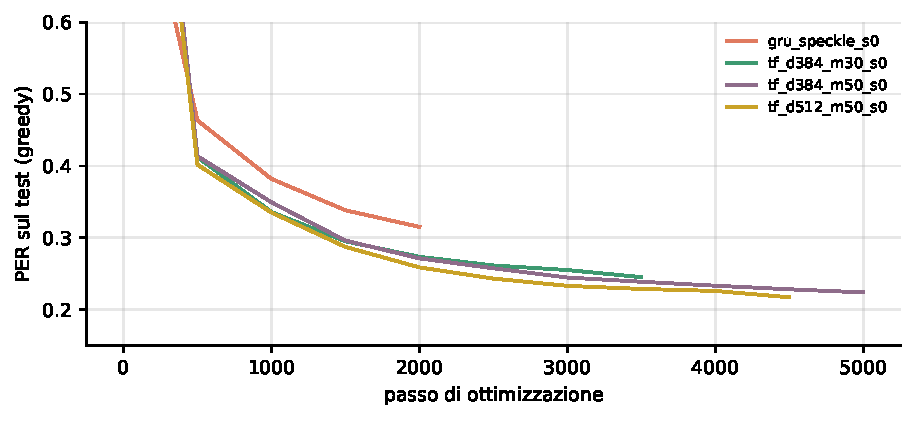
\includegraphics[width=0.9\linewidth]{training_curves.pdf}
\caption{PER sul test durante l'addestramento dei primi quattro decoder, in corso al momento della stesura. \texttt{tf\_d384\_m50}: Transformer con $d=384$ e il 50\% del tempo mascherato. \texttt{gru\_speckle}: GRU bidirezionale con speckle masking. Per costruzione il GRU è più lento per passo.}
\label{fig:curves}
\end{figure}


\paragraph{Prima decodifica completa.} Per verificare la pipeline da un capo all'altro abbiamo esportato un checkpoint intermedio del Transformer (\texttt{tf\_d384\_m50} al passo 2500, PER greedy 25{,}8\%) e lo abbiamo decodificato con il 5-gram. Sul test il WER 1-best è del \textbf{25{,}9\%}, ancora senza rescoring LLM, con i parametri di decodifica della baseline ($\lambda=0{,}5$, penalità di blank $\log 7$) e con un modello fermo al passo 2500 di 20\,000. Non è un risultato competitivo: serve a confermare che tutti i componenti funzionano insieme. La Tab.~\ref{tab:esempi} mostra alcune frasi decodificate.

Dagli esempi si vede come lavora il modello linguistico. Per la frase \emph{``i'm sure there are some''} la decodifica greedy produce i fonemi
\begin{center}\small\texttt{AY M | SH UH R | DH EH R | AW R | T AY M |}\end{center}
(\texttt{|} indica la fine di una parola). La sequenza contiene errori (\texttt{AW R} per \emph{are}, \texttt{T AY M} per \emph{some}), ma il 5-gram li corregge e restituisce la frase esatta. Quando invece gli errori fonetici sono molti, il 5-gram sceglie una frase plausibile in inglese ma sbagliata (\emph{``spinal tap''} per \emph{``financial type''}): è proprio il caso in cui contano un decoder neurale migliore, un LLM che guardi tutta la frase e l'ensemble.

\begin{table}[h]
\centering\small
\begin{tabularx}{\linewidth}{>{\raggedright\arraybackslash}X >{\raggedright\arraybackslash}X c}
\toprule
\textbf{Frase pronunciata (riferimento)} & \textbf{Decodifica neurale + 5-gram} & \\
\midrule
\textit{that stinging vapor was caused by chloride vaporization} & that thing as it was called was called up in &  \\
\textit{a sharp tremor was followed by a jerky roll} & a top team with killed by a truck while &  \\
\textit{that's a science in itself} & that's a science in itself & \checkmark \\
\textit{i'm sure there are some} & i'm sure there are some & \checkmark \\
\textit{most people aren't} & more people want &  \\
\textit{it's a little bit financial type thing} & it's a little bit spinal tap thing &  \\
\bottomrule
\end{tabularx}
\caption{Esempi reali dalla partizione di test, decodificati dal checkpoint intermedio con il 5-gram (ipotesi migliore su 100), senza rescoring LLM.}
\label{tab:esempi}
\end{table}

\begin{table}[h]
\centering\small
\begin{tabular}{lcc}
\toprule
\textbf{Sistema} & \textbf{WER} & \textbf{Fonte} \\
\midrule
Baseline NPTL: RNN + 5-gram + OPT & 9{,}76\% & classifica EvalAI \\
DCoND-LIFT, vincitore 2024 (ensemble + GPT-3.5 addestrato) & 5{,}77\% & classifica, arXiv:2411.10657 \\
Miglior metodo pubblicato (LightBeam) & 4{,}98\% & classifica, arXiv:2603.14002 \\
Primo classificato (metodo non pubblicato) & 2{,}99\% & classifica, 22/11/2026 \\
\midrule
Questo lavoro: checkpoint intermedio + 5-gram (sul test) & 25{,}9\% & questo documento \\
\bottomrule
\end{tabular}
\caption{Contesto: i numeri della classifica sono misurati sulla partizione di gara, il nostro sul test. I due valori non sono direttamente confrontabili.}
\label{tab:classifica}
\end{table}


\section{Infrastruttura}

\begin{itemize}\setlength\itemsep{0pt}
\item \textbf{Server:} un server di ateneo con 64 thread CPU, 372\,GB di RAM e due NVIDIA Tesla T4 da 16\,GB.
\item \textbf{Esecuzione:} tutto gira in sessioni \texttt{screen} indipendenti.
\item \textbf{Addestramento:} una coda di job su file alimenta quattro worker, due per GPU. Se un job va in out-of-memory viene rimesso in coda.
\item \textbf{Decodifica:} un servizio carica il 5-gram una sola volta e decodifica automaticamente ogni nuovo modello.
\item \textbf{Orchestrazione:} un orchestratore accoda il rescoring LLM e produce il file di sottomissione.
\item \textbf{Vincoli:} il driver CUDA 12.2 impone PyTorch 2.7, e il decoder WFST (C++, WeNet e Kaldi) usa un ambiente Python separato con libtorch 1.13.
\end{itemize}

\section{Limiti e prossimi passi}

\begin{itemize}\setlength\itemsep{1pt}
\item \textbf{Validazione.} Il test (880 frasi) serve sia a scegliere gli iperparametri sia a stimare il WER, quindi la stima è ottimista. Le sottomissioni a EvalAI (cinque al giorno) sono l'unica misura imparziale.
\item \textbf{Metodi dei primi classificati.} I primi tre non hanno pubblicato il metodo. Il miglior risultato con metodo pubblicato è 4{,}98\%: scendere sotto il 3\% richiede di andare oltre lo stato dell'arte pubblicato.
\item \textbf{Sviluppi possibili:}
  \begin{itemize}\setlength\itemsep{0pt}
  \item target a difoni (DCoND);
  \item pre-addestramento su altri dataset pubblici di speech BCI, per esempio il partecipante T15 della gara 2025;
  \item adattamento non supervisionato sui giorni della partizione di gara (\emph{test-time adaptation});
  \item un LLM di fusione più grande.
  \end{itemize}
\end{itemize}

\paragraph{Riferimenti principali.}
\begin{itemize}\setlength\itemsep{0pt}
\item F.\,R.\ Willett et al., \emph{A high-performance speech neuroprosthesis}, Nature 620 (2023).
\item F.\,R.\ Willett et al., \emph{Brain-to-Text Benchmark '24: lessons learned}, arXiv:2412.17227.
\item A.\ Graves et al., \emph{Connectionist Temporal Classification}, ICML 2006.
\item J.\ Li et al., \emph{DCoND-LIFT}, arXiv:2411.10657.
\item E.\ Feghhi et al., \emph{Time-masked Transformers for speech BCI}, arXiv:2507.02800.
\end{itemize}

\end{document}
